\section{Introducción}

\PARstart 
En el modelo OSI, la capa de enlace es la responsable de la transferencia fiable
de información a través de un circuito de transmisión de datos. Recibe peticiones de
una capa superior (la capa de red) y utiliza los servicios de la capa física (primer
capa). 
\begin{figure}[h]
  \centering
    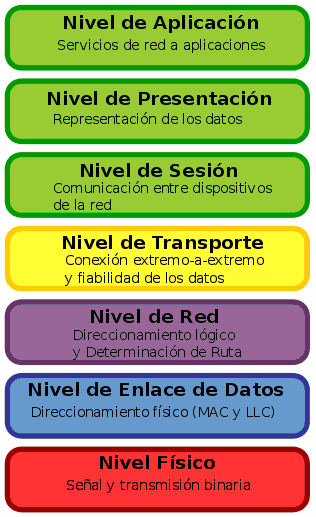
\includegraphics[width=0.2\textwidth]{modeloOSI.png}
  \caption{}
  \label{}
\end{figure}
\\
ARP es un protocolo que se encarga de ser el nexo entre la capa de enlace y la capa de red. 
Su tarea es poder asociar direcciones IP (obtenidas por algún medio externo) con la dirección MAC (Media Access Control).
A nivel teórico, es una suerte de protocolo se encarga de encontrar la dirección MAC que corresponde a una IP determinada.
Para lograr dicho objetivo, un host emite un paquete en la red con dirección broadcast (ARP request) preguntando
por una IP específica esperando por la respuesta (ARP reply) de algún host conectado a esa red. 


Los paquetes ARP tienen el siguiente formato:
\begin{figure}[!h]
  \centering
    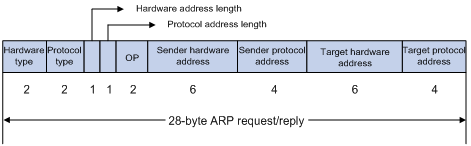
\includegraphics[width=0.45\textwidth]{arpPacket.png}
  \caption{}
  \label{}
\end{figure}
\\
Cuando un host A emite un paquete ARP request y luego el host B con dirección IP igual a la requerida por el host B
responde con el paquete ARP reply, el host A se guarda en una tabla de cache la dirección MAC del host B.
Sin embargo la tabla se elimina cada cierto tiempo ya que las direcciones pueden cambiar.

Nuestro objetivo será construir herramientas que nos permitan analizar este tráfico,
mas específicamente los mensajes ARP request de los hosts conectados a una red no trivial.
